\subsection{Overview}
	Here we provide a high level representation of client-server interaction and of the submodule of the server.
	The orchestrator is needed only during the creation of the communication: his role is to dispatch the request of the client to the appropriate component. After that, the component can communicate directly with the client and vice versa.\newline
	In the server, the orchestrator and all the submodules are stateless. We thought to use the elastic component architectural pattern for the components. Moreover, the orchestrator can eventually be duplicated using a fixed dimension pool whose size is configurable by the system administrator.\newline
	Further details on the submodule and the overall interaction will be provided in the next sections.

	\begin{figure}[H]
		\centerline{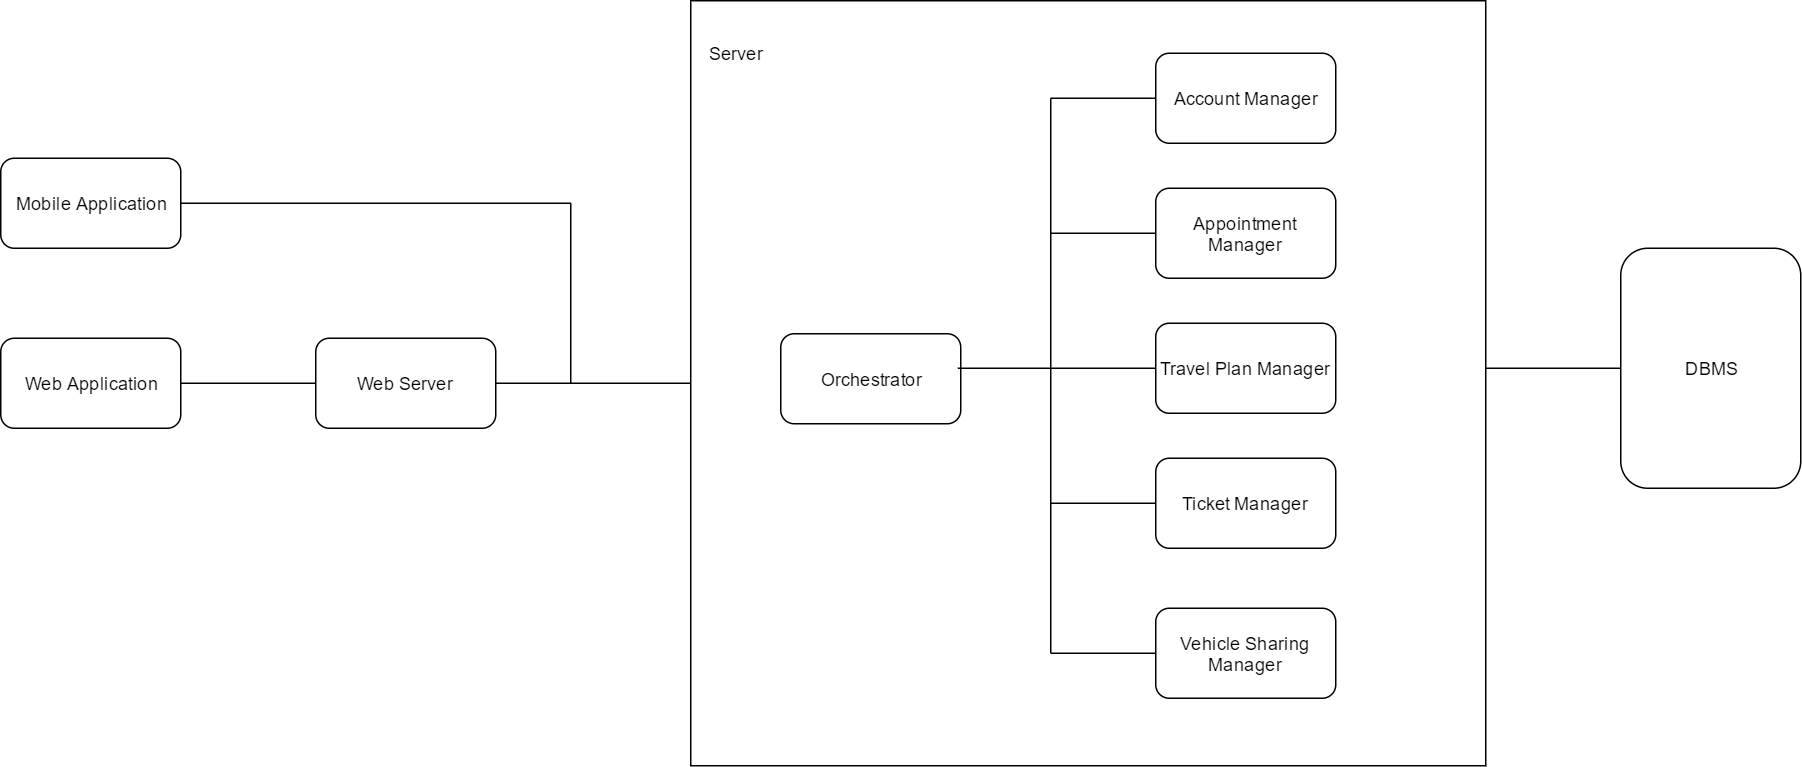
\includegraphics[width=0.9\paperwidth]{Images/HighLevelArchitecture}}
		\caption{High level Architecture Diagram - Client-Server interaction}
	\end{figure}

\filbreak
\subsection{Component view}
	This section starts with the presentation of the Entity Relationship diagram. In the other diagram following ER model, we include a fictitious component, App, that will be highlighted in green and serves the purpose of representing both the mobile app and the web app (through the web server), without adding complexity to the diagrams.
	\subsubsection{ER diagram}
	The following ER diagram represents the conceptual schema of the system database. In Ticket entity we don't specify all the attributes because they depend from ticket Typology and from Transportation Company they belong. Ticket entity can be split into two categories of tickets, ordinary and pass tickets. Below these two, we have another hierarchy in which we include some examples.
	
    \begin{figure}[H]	
		\centerline{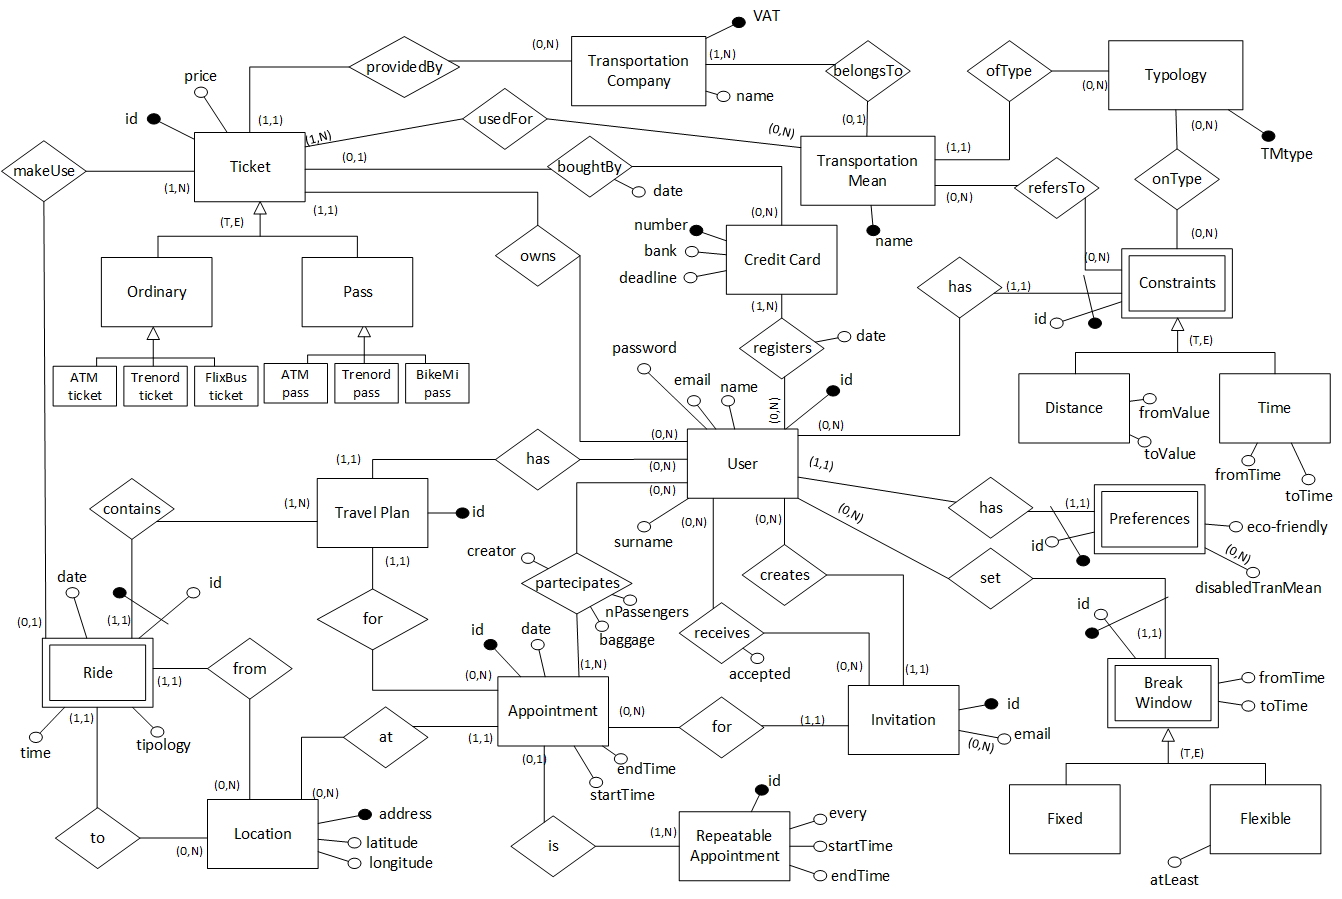
\includegraphics[width=0.9\paperwidth]{Images/ERdiagram}}
		\caption{ER diagram}
 	\end{figure}

	\filbreak
	\subsubsection{Appointment Manager and Notification Manager}
		\label{sect:AppointmentManager}
		\label{sect:NotificationManager}
		Here we define the Appointment Manager and the Notification Manager. The Notification Manager will appear in others diagrams, but only here is detailed with its subcomponents. 
		\medskip\newline
		Appointment Manager has three subcomponents:		
		\begin{description}[before={\renewcommand{\makelabel}[1]{-- \textit{##1}:}}]
			\item[Appointment Handler] it is the only subcomponents communicating with the database: it manages all the read and write operations related to appointments. It is responsible for the final consistency check of the appointment before writing it to database. It exports an interface to let external components read appointments details and an internal interface to let subcomponents of Appointment Manager read and write appointments' details.
			\item[Appointment Editor] this provides an interface to easily change appointments' details and store it to database through the interface of Appointment Handler. Every time an appointment is created or details of an appointment changes, this send to Incoming Appointment Scheduler the appointment. This module interacts with an external module "Solution Calculator" to compute travel solutions. In this diagram it is displayed in dashed line because it will be described in another diagram.
			\item[Incoming Appointment Scheduler] for each appointment (provided by Appointment Editor) this module executes an algorithm to decide when that specific appointment will become an \defined{incoming appointment}. An appointment becomes incoming according to a combination of the time of the appointment and the travel plan chosen, to let the User receive a notification at an appropriate time. This is done generating a \defined{future notification} through the interface provided by Notification Manager.
		\end{description}
		\bigskip
		Notification Manager provide an interface for the creation of new notification and it is composed by two module:
		\begin{description}[before={\renewcommand{\makelabel}[1]{-- \textit{##1}:}}]
			\item[Notification Scheduler] this is the module whose interface is actually exported and it manages the creation of new notifications, stores them in the database and schedules their dispatch. When it is time to send a notification this module uses the interface provided by Notifier and delegate to it the dispatching procedure.
			\item[Notifier] it is in charge of the actual dispatch of the notification.
		\end{description}
		
		\begin{figure}[H]	
			\centerline{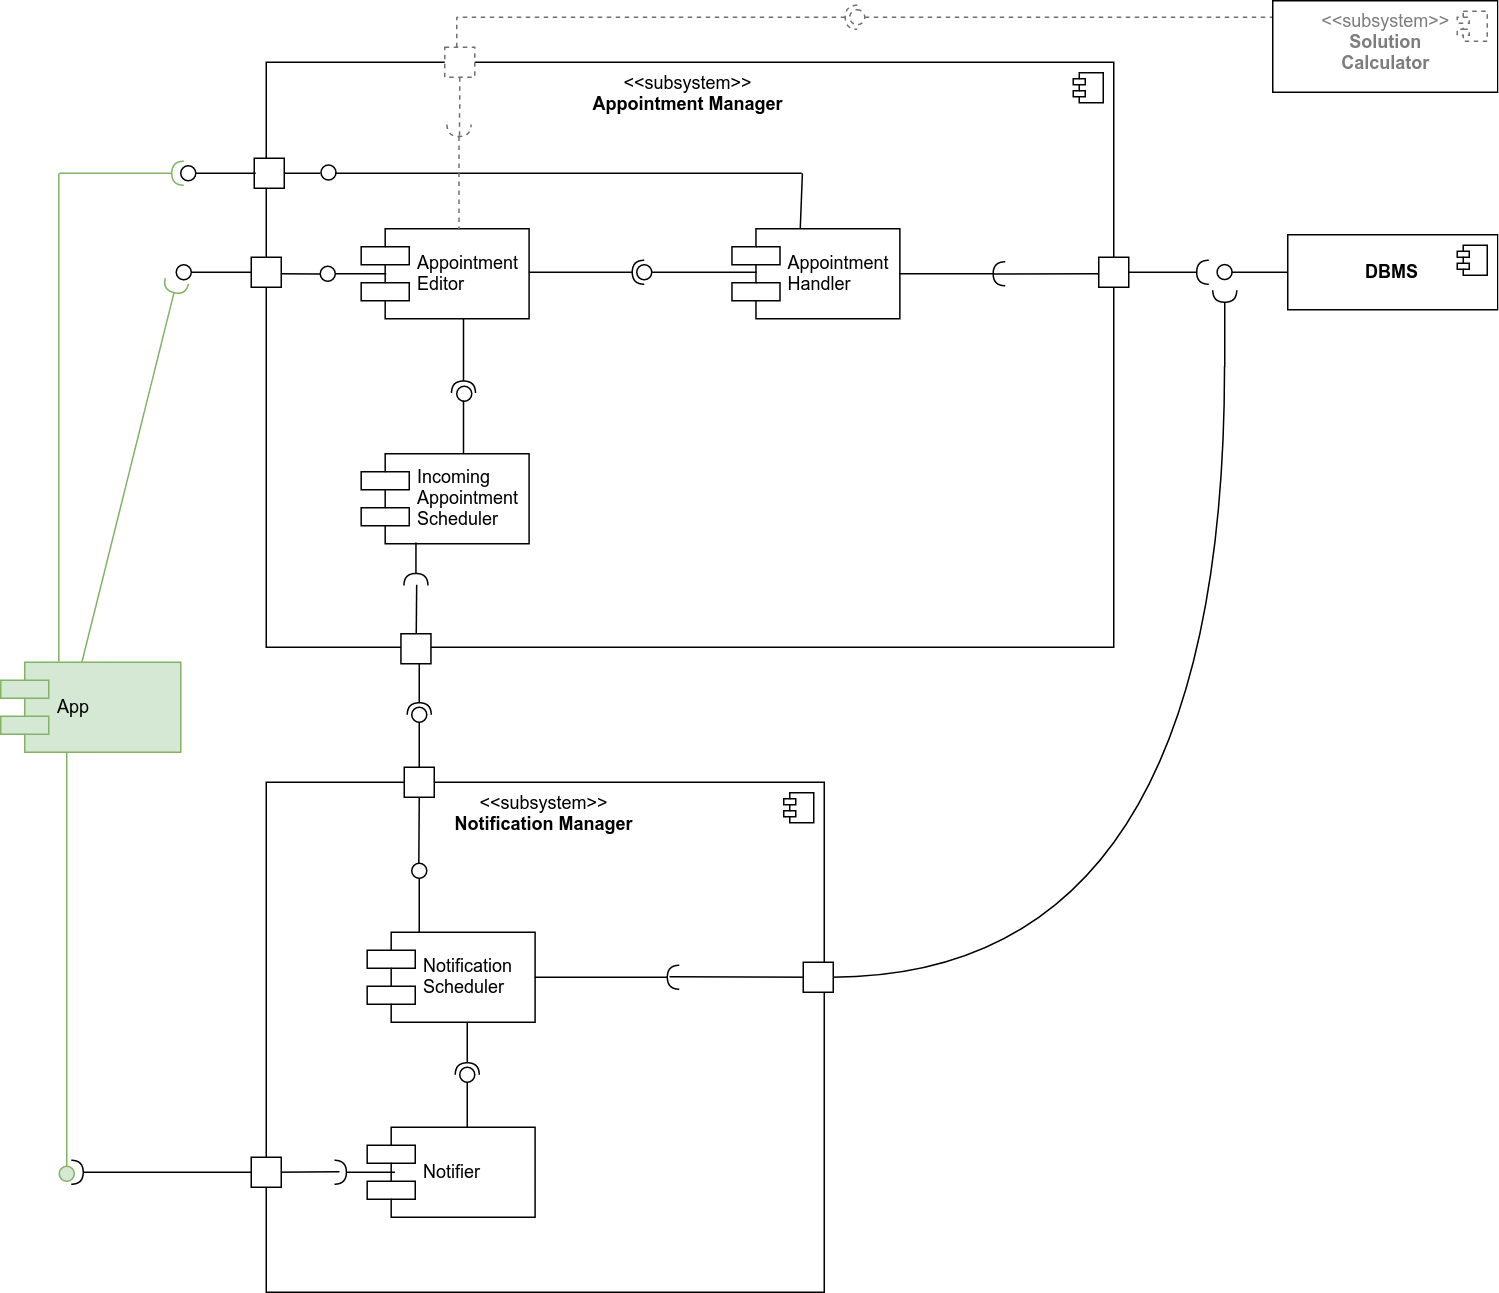
\includegraphics[width=0.9\paperwidth]{Images/CD_AppointmentManager}}
			\caption{Component Diagram - Appointment Manager \& Notification Manager}
		\end{figure}
		
	\filbreak
	\subsubsection{Invitation Manager}
		\label{sect:InvitationManager}
		The Invitation Manager component is the module that manages all the aspects related to invitations, from their creation to the acceptance/refusal of the invited Users/Persons. It is divided into two subcomponents. A sequence diagram is provided in section \ref{sect:RuntimeView}.
		\begin{description}[before={\renewcommand{\makelabel}[1]{-- \textit{##1}:}}]
			\item[Invitation Generator] it manages the creation of a new invitations 
			\item[Invitation Handler] it is concerned with the acceptance/refusal of the invitations sent.
		\end{description}
		
		\begin{figure}[H]	
			\centerline{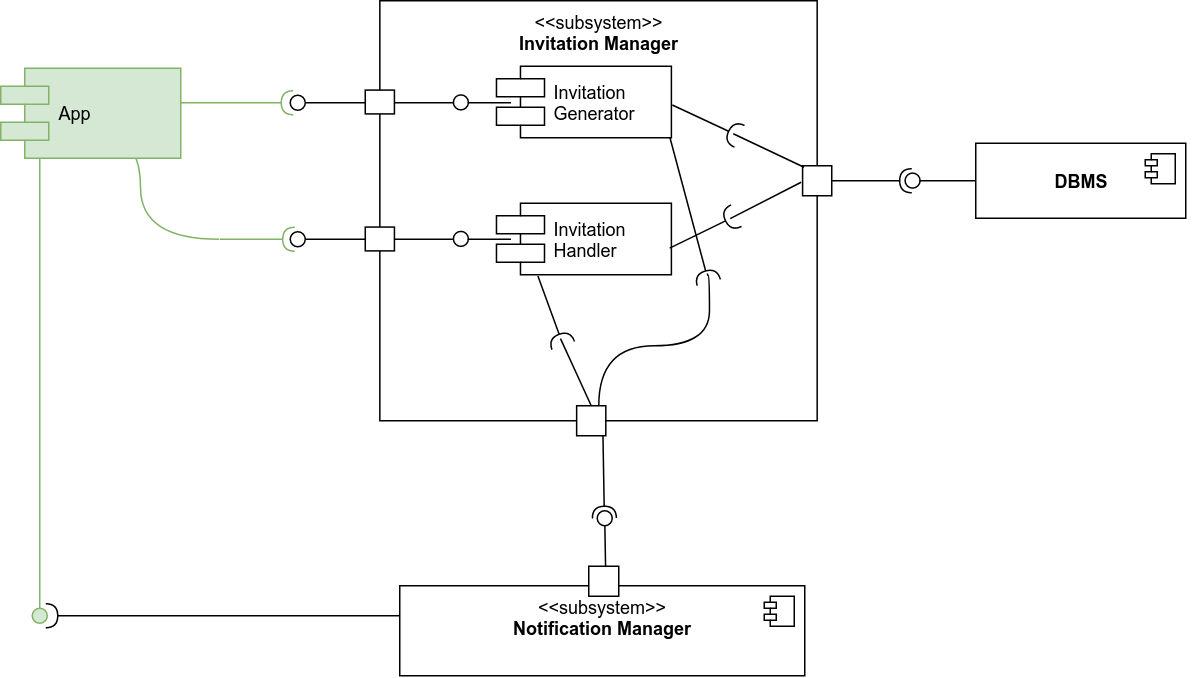
\includegraphics[width=0.9\paperwidth]{Images/CD_InvitationManager}}
			\caption{Component Diagram - Invitation Manager}
		\end{figure}
	
	\filbreak
	\subsubsection{Weather and Traffic Modules}
		\label{sect:WeatherTrafficModules}
		In the diagram, we provide the representation of the Weather Module. The traffic module has exactly the same architecture and interactions. You can just derive the traffic diagram substituting \textit{"Weather"} with \textit{"Traffic"}. Both modules are needed to notify the User of changes in traffic/weather that can influence his/her daily travels and they are used by the component Solution Calculator to avoid bad solutions like, for instance, taking the bike when it rains. With the same convention as before, we represent here Solution Calculator but it will be detailed in another diagram.\newline
		The Weather \textit{(traffic)} module has a quite articulated architecture and it will be explained here and in section \ref{sect:RuntimeView} with an object diagram.\newline
		It is composed by:
		\begin{description}[before={\renewcommand{\makelabel}[1]{-- \textit{##1}:}}]
			\item[Address Solver] this component has a really basic functionality and it is exploited by Weather Manager to "understand" \textit{(see below)} addresses. Provided an address as input, it decompose it in its components and return a hierarchy.\newline
			Example: "Italy, Milan, via Pacini 32" -> transformed to:\newline "State:Italy"$\rightarrow$"City:Milan"$\rightarrow$"CityZone:NorthEast"$\rightarrow$"Street:Giovanni Pacini"$\rightarrow$"Number:32"
			\item[Weather Manager] this serves as a registry to support the publish-subscribe architecture between Weather Querier and Weather Notifier. Moreover, this component provides an external interface to let other components have information about weather. When it receives a request of weather information for a specific address, it asks Address Solver to interpret the address and then it asks the appropriate Weather Querier for the information.
			\item[Weather Querier] it is the module responsible for retrieving the weather information and send them to the Weather Notifier.
			\item[Weather Notifier] this is the component that decides if and when a User has to be notified. It subscribes to a specific Weather Querier and receives the information from it. 
		\end{description}
		\medskip
		Both the Querier and the Notifier are instantiated by zone. The zone of the Querier are meant to be very wide, like Italy, Spain, France and the zone of the Notifier are meant to be more specific, for instance: West Milan, East Milan, Venice, Turin.\newline
		The Notifier has to execute an algorithm for each appointment to decide if and when to notify the User, so its load will depend on the number of appointments in that specific zone and (especially in the Traffic Module) on the day of the week and the time of the day. For this reason, a load balancing mechanism is required. When a 'node' is under load it can be splitt into two or more parts: "Milan"$\rightarrow$"WestMilan" and "EastMilan".\newline
		The Querier has a more stable load and, for this reason, \textbf{no} load balancing mechanism has to be implemented. By the way, the zones of the Querier can be configured by the System Administrator, even dynamically.\newline
		The load balancing mechanism of the Notifier and the \defined{dynamically configurable} Querier has to be supported by the Manager: it is not a simple registry but it registers all the active Queriers and Notifiers and it manages the subscriptions when they are modified.\newline
		The process is described in more details in section \ref{sect:algorithmDesign}.

		\begin{figure}[H]
			\centerline{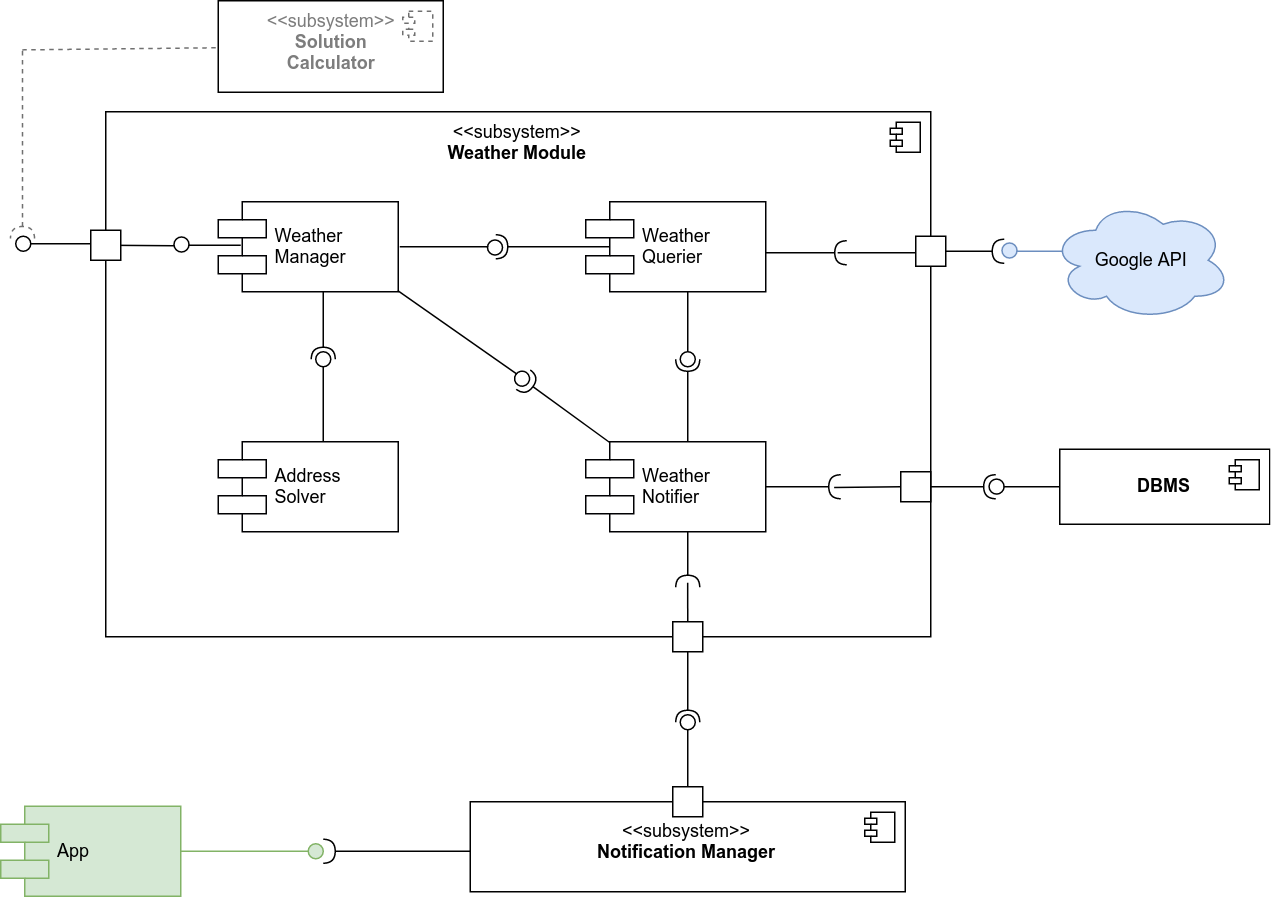
\includegraphics[width=0.9\paperwidth]{Images/CD_WeatherModule}}
			\caption{Component Diagram - Weather Module}
		\end{figure}

	\filbreak
	\subsubsection{Ticket Manager}
		\label{sect:TicketManager}
		Ticket Manager role is to handle the process that goes from the User selection of a travel plan solution to the purchase or the registration of a ticket.\newline
		It is composed by:
		\begin{description}[before={\renewcommand{\makelabel}[1]{-- \textit{##1}:}}]
			\item[Ride Controller] it receives the travel plan selected by the User and, for each ride, checks if it contains a transportation mean of an affiliated company which requires tickets. Ride controller forwards to Purchase Manager all the rides for which the User could buy a ticket.
			\item[Purchase Manager] it provides to the User the list of possible tickets to purchase. The DB contains only the ticket models of the affiliated transportation companies, so it could be necessary to interface with the Transportation Companies API in order to obtain, in real time, additional information about the ride (e.g., number of available seats, departure time, etc.). For instance, if we need an ATM bus ticket, Purchase Manager takes it from the DB, because the ticket model is enough (for this kind of ticket we don't need to specify departures time or seat number); at the contrary, if we need a Trenitalia ticket, Purchase Manager interfaces with the Transportation Companies API to obtain, in real time, all the necessary information. \newline
			Purchase Manager role is also to register into the DB an eventual pass bought by User externally from the system.
			\item[Payment Handler] it handles the phase in which the User chooses the ticket and proceeds to the payment. It interfaces with the DB to have information about User's credit cards data and also with the Transportation Companies API, in order to forward the payment.  
		\end{description}

		\begin{figure}[H]
			\centerline{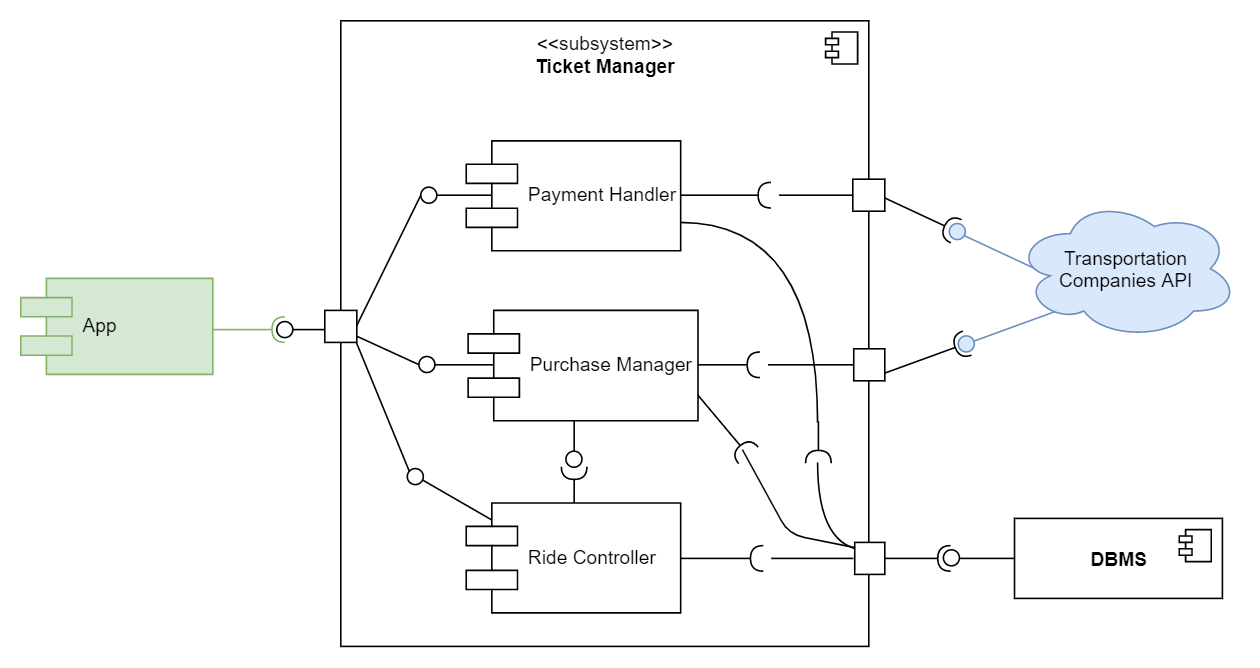
\includegraphics[width=0.9\paperwidth]{Images/CD_TicketManager}}
			\caption{Component Diagram - Ticket Manager}
		\end{figure}

\subsection{Deployment view}
	% TODO
	
\subsection{Runtime view}
	\label{sect:RuntimeView}
	\subsubsection{Sequence Diagram - Sign Up}
	\label{sect:sd_signUp}
	\begin{figure}[H]
		\centerline{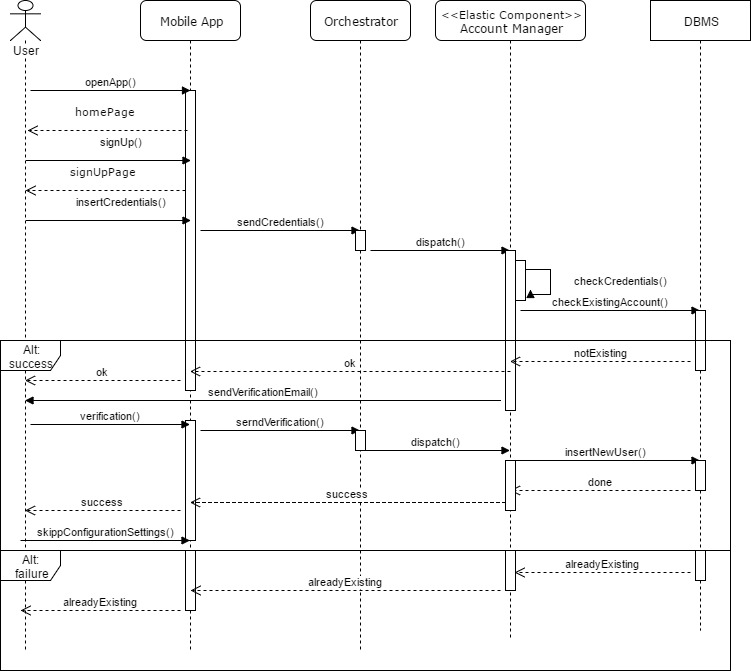
\includegraphics[width=0.9\paperwidth]{Images/signUp}}
		\caption{Sequence Diagram - SignUp}
	\end{figure}
	
	\subsubsection{Sequence Diagram - Modify Settings}
	\begin{figure}[H]
		\centerline{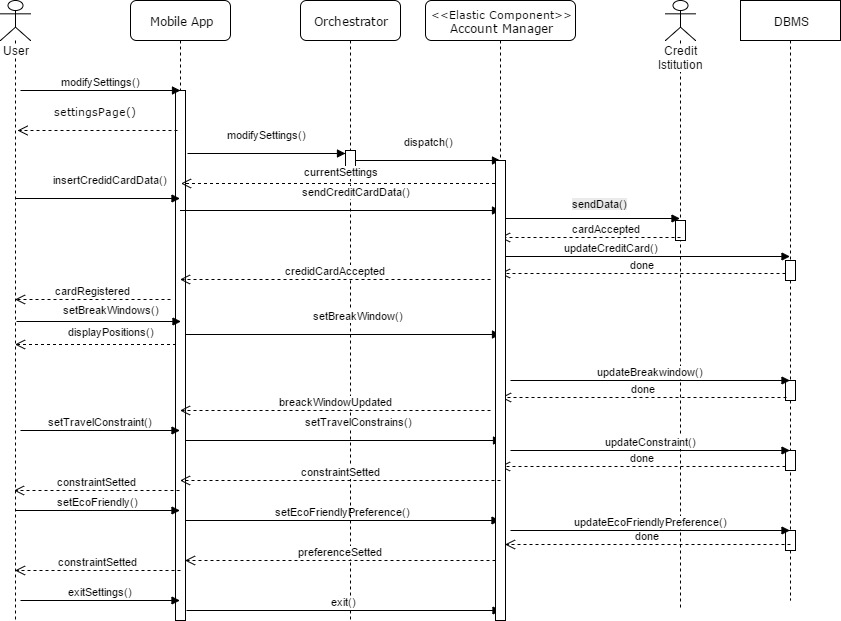
\includegraphics[width=0.9\paperwidth]{Images/ModifySettings}}
		\caption{Sequence Diagram - Modify Settings}
	\end{figure}

	\subsubsection{Sequence Diagram - Invitation Creation}
		\begin{figure}[H]
			\centerline{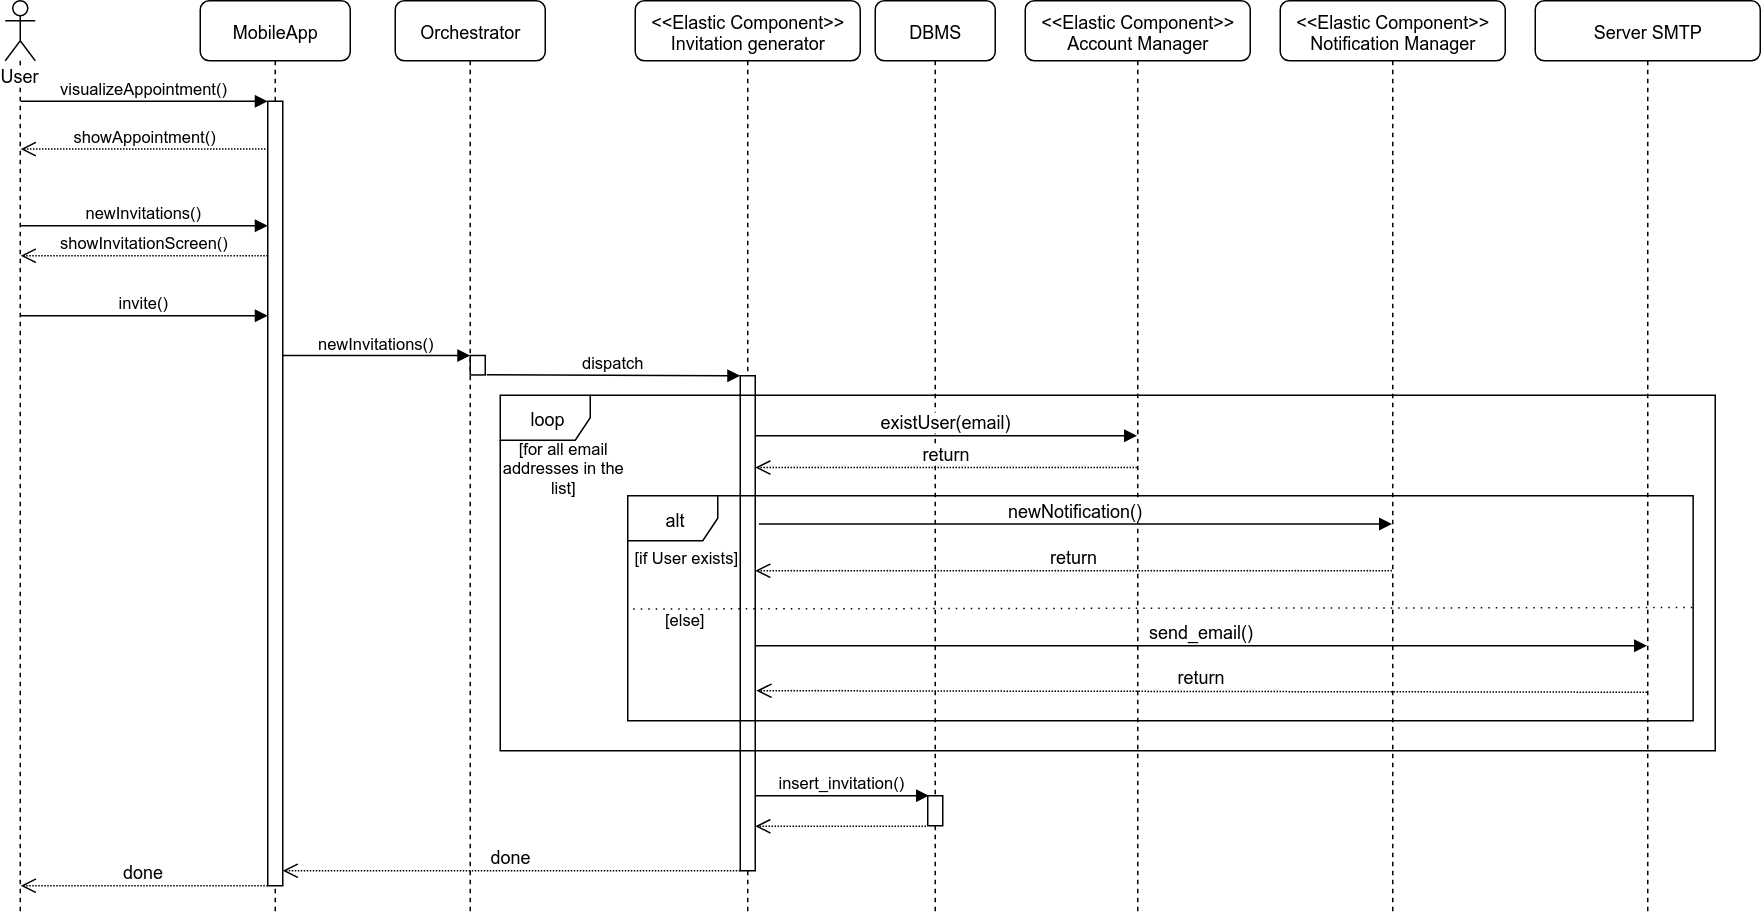
\includegraphics[width=0.9\paperwidth]{Images/SD_InvitationCreation}}
			\caption{Sequence Diagram - Invitation Creation}
		\end{figure}
	\subsubsection{Sequence Diagram - Select TravelPlan Solution}
		\label{sect:Select TravelPlan Solution}
		\begin{figure}[H]
			\centerline{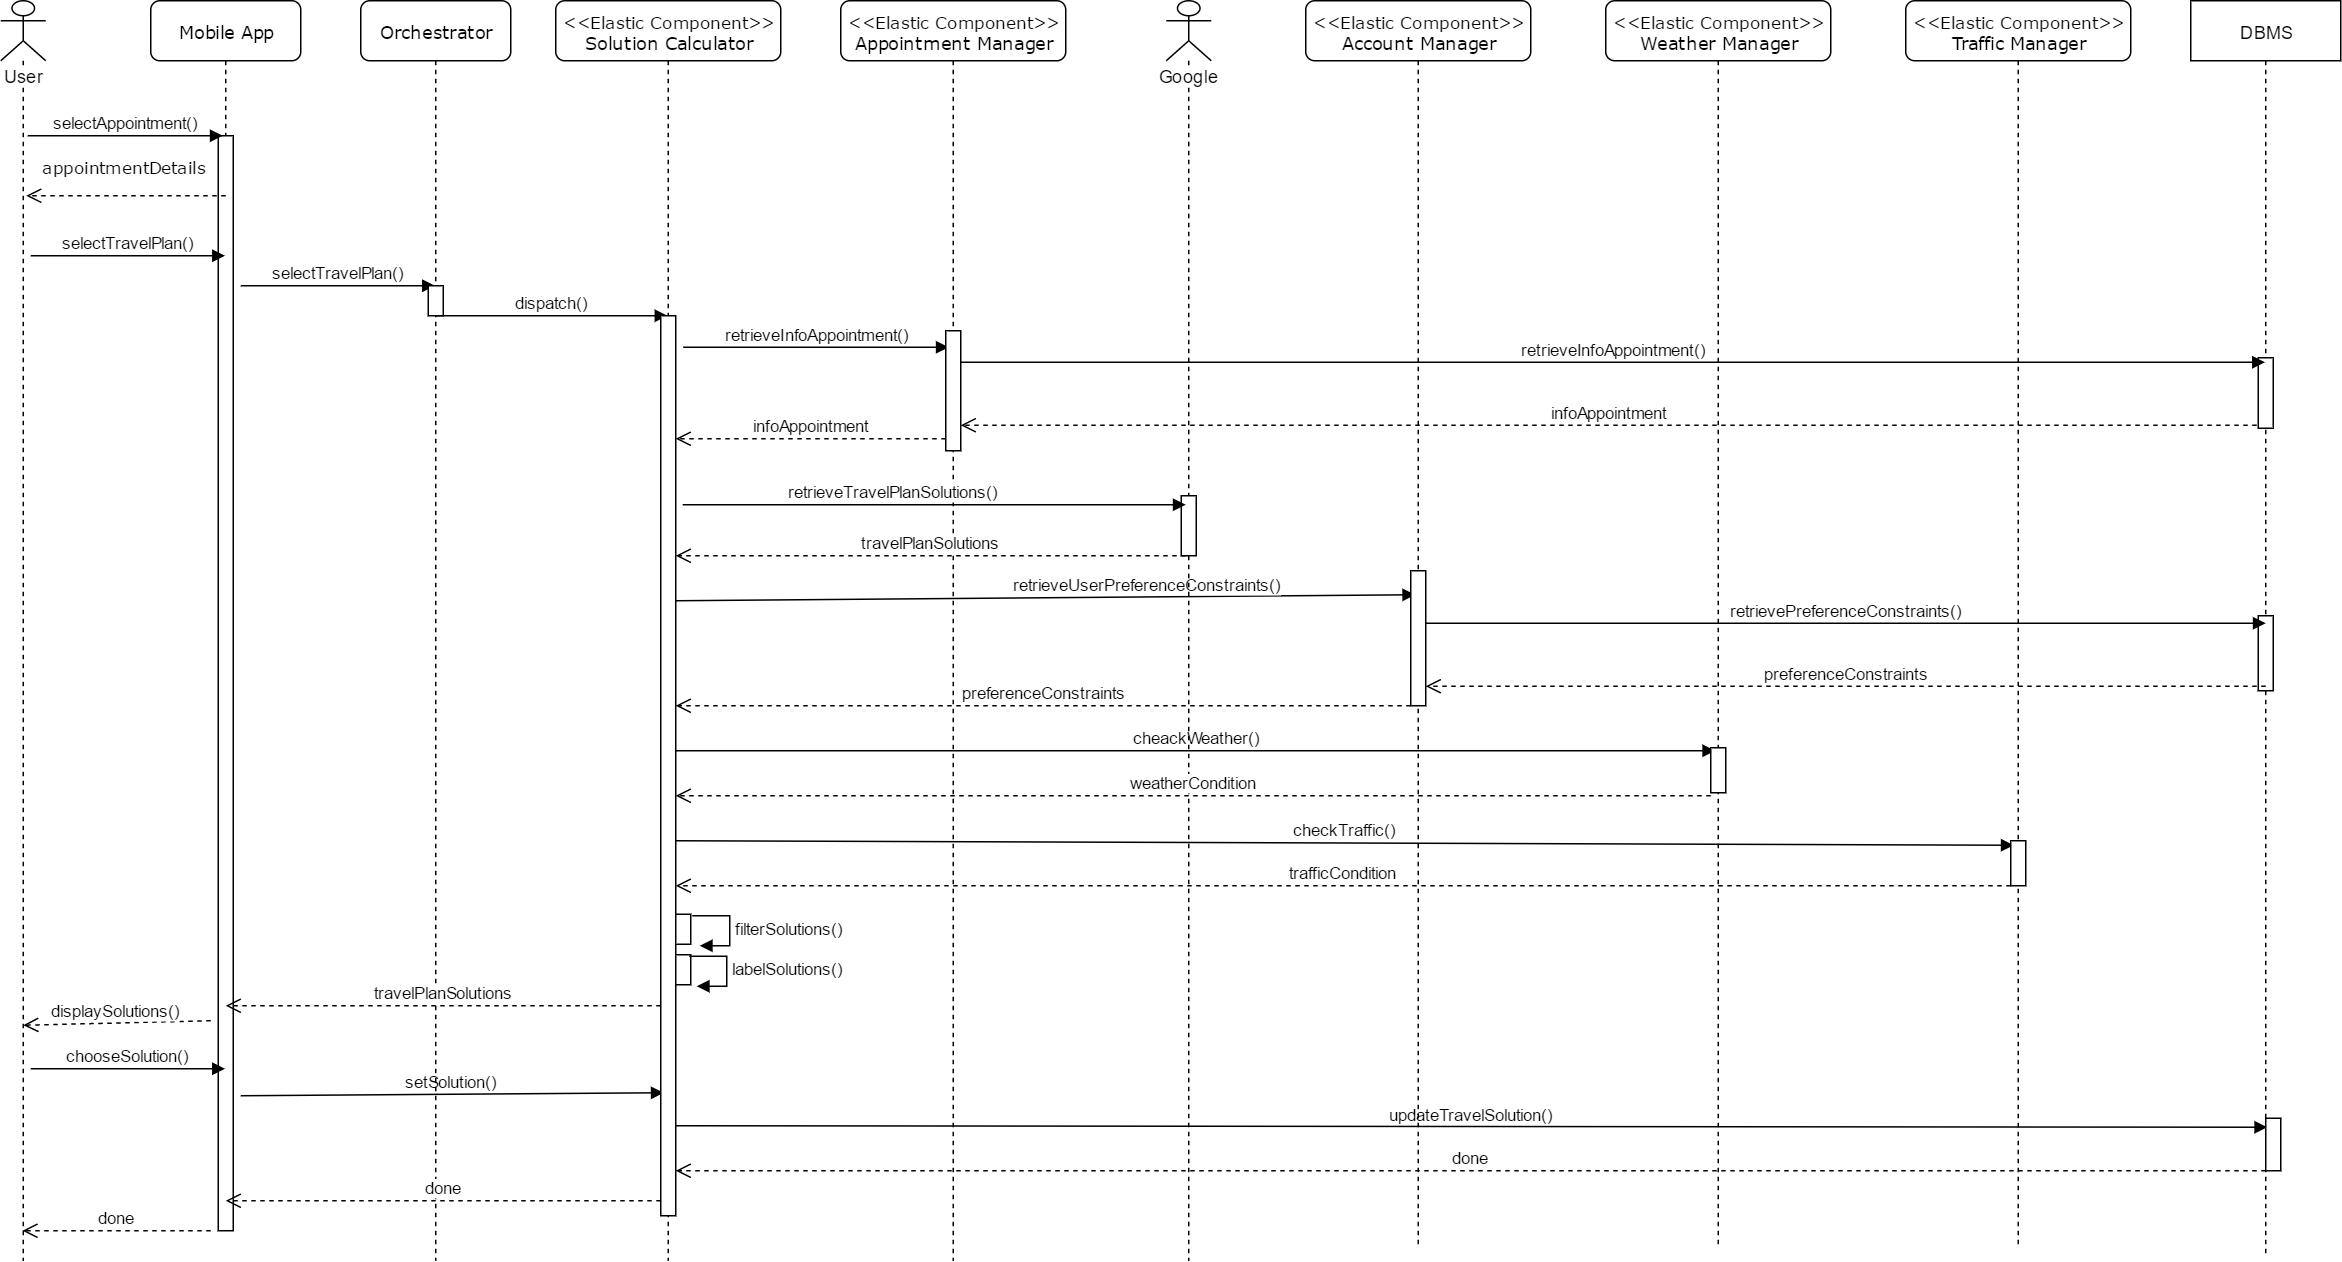
\includegraphics[width=0.9\paperwidth]{Images/selectTravelSolution}}
			\caption{Sequence Diagram - Select TravelPlan Solutions}
		\end{figure}
	\subsubsection{Sequence Diagram - Locate Nearest Vehicle}
		\begin{figure}[H]
			\centerline{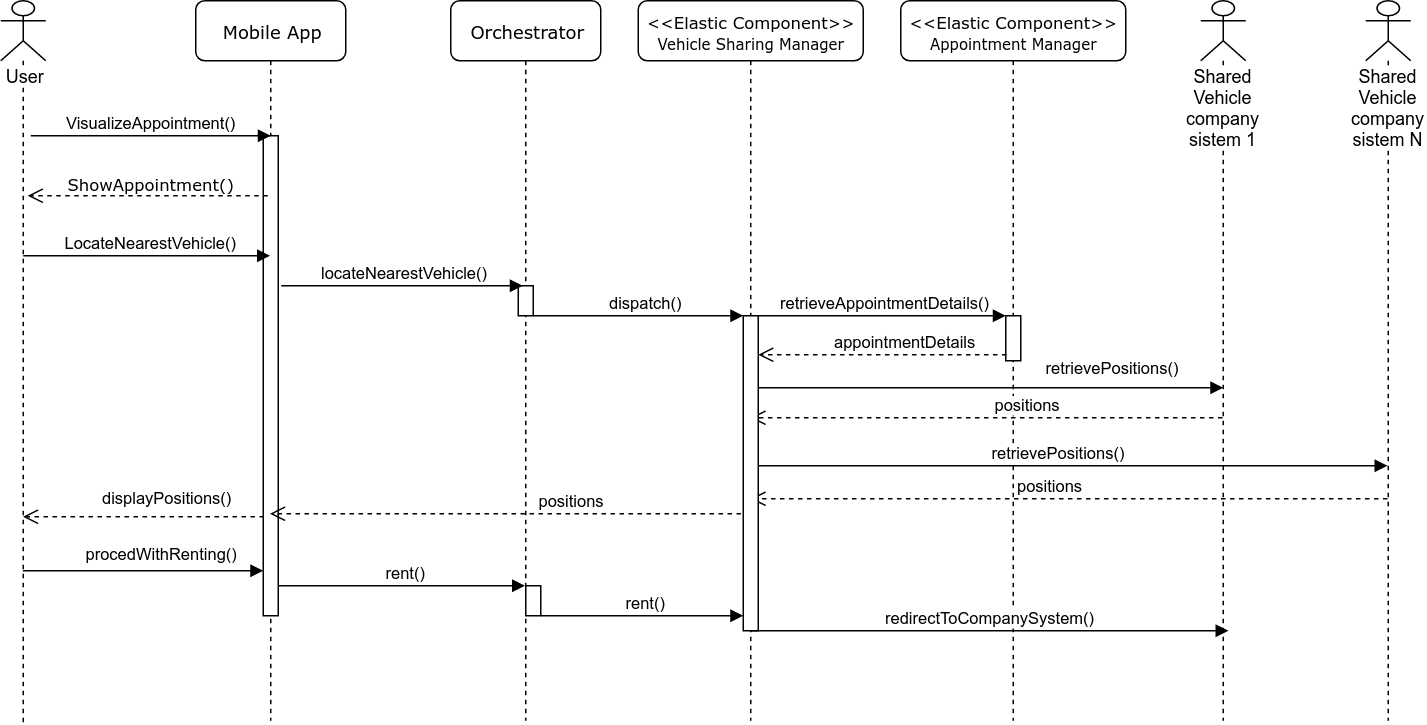
\includegraphics[width=0.9\paperwidth]{Images/LocateNearest}}
			\caption{Sequence Diagram - Locate Nearest Vehicle}
		\end{figure}
		
	\subsubsection{Object Diagram - Weather \& Traffic Modules}
		As said in the component diagram \hyperref[sect:WeatherTrafficModules]{description}, this architecture is exactly the same used in the Traffic Module and so we provide here only the object diagram of one of them, the Weather Module, for consistency with the component diagram.\newline
		The two diagrams illustrate an evolution in the instances caused by a load balancing operation and an unexpected crash. Both diagrams are not complete of all the instances and we used dashed lines to represent the fact that some instances have been cut, to have simpler and easier to understand diagrams.\newline
		In the first diagram, we can see two Querier, one for Italy and one for France. This partition of the region have been chosen by the System Administrator (another option could have been Europe). The Querier are linked to the related Notifiers and to the Manager. The Manager keeps track of the Queriers, the active Notifiers and the Notifiers in the standby list.
		\begin{figure}[H]
			\centerline{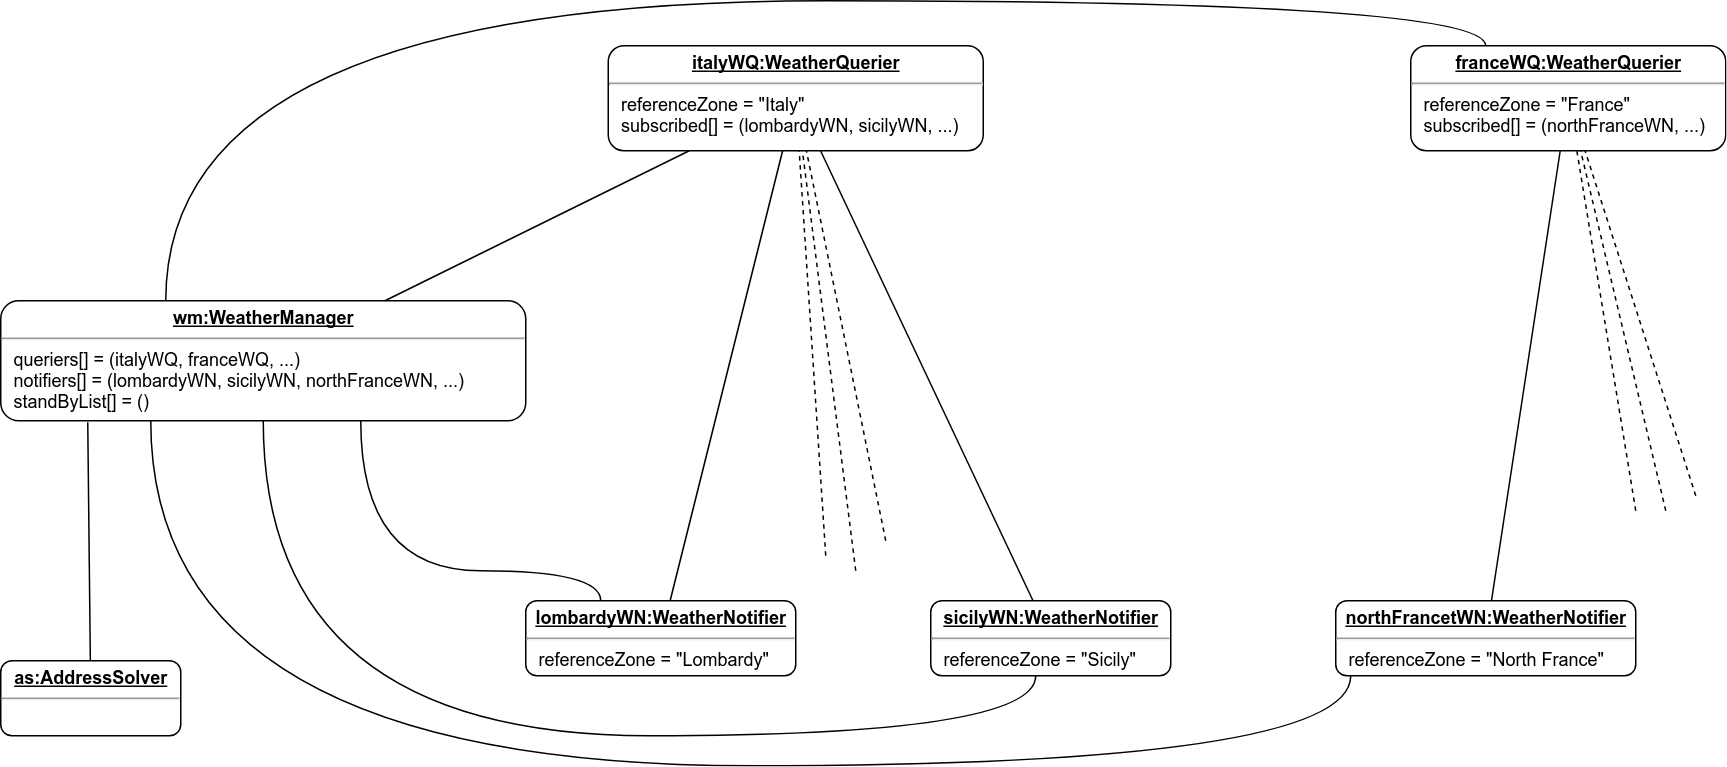
\includegraphics[width=0.9\paperwidth]{Images/OD_WeatherModule_Before}}
			\caption{Object Diagram - Weather Module Original State}
		\end{figure}
		\noindent
		At some point, the Notifier related to Lombardy is under load and the load balancer split it into two Notifiers, respectively related to North Lombardy and South Lombardy. Their subscription to the Querier \inlinecode{italyWQ} is managed directly by the Manager as described in algorithm section (\ref{sect:WeatherTrafficAlgorithm}).\newline
		The \inlinecode{franceWQ} Querier unexpectedly crashes and the Notifiers that were subscribed to it are put in the standby list by the Manager.\newline
		The next diagram represents the final situation.
		\begin{figure}[H]
			\centerline{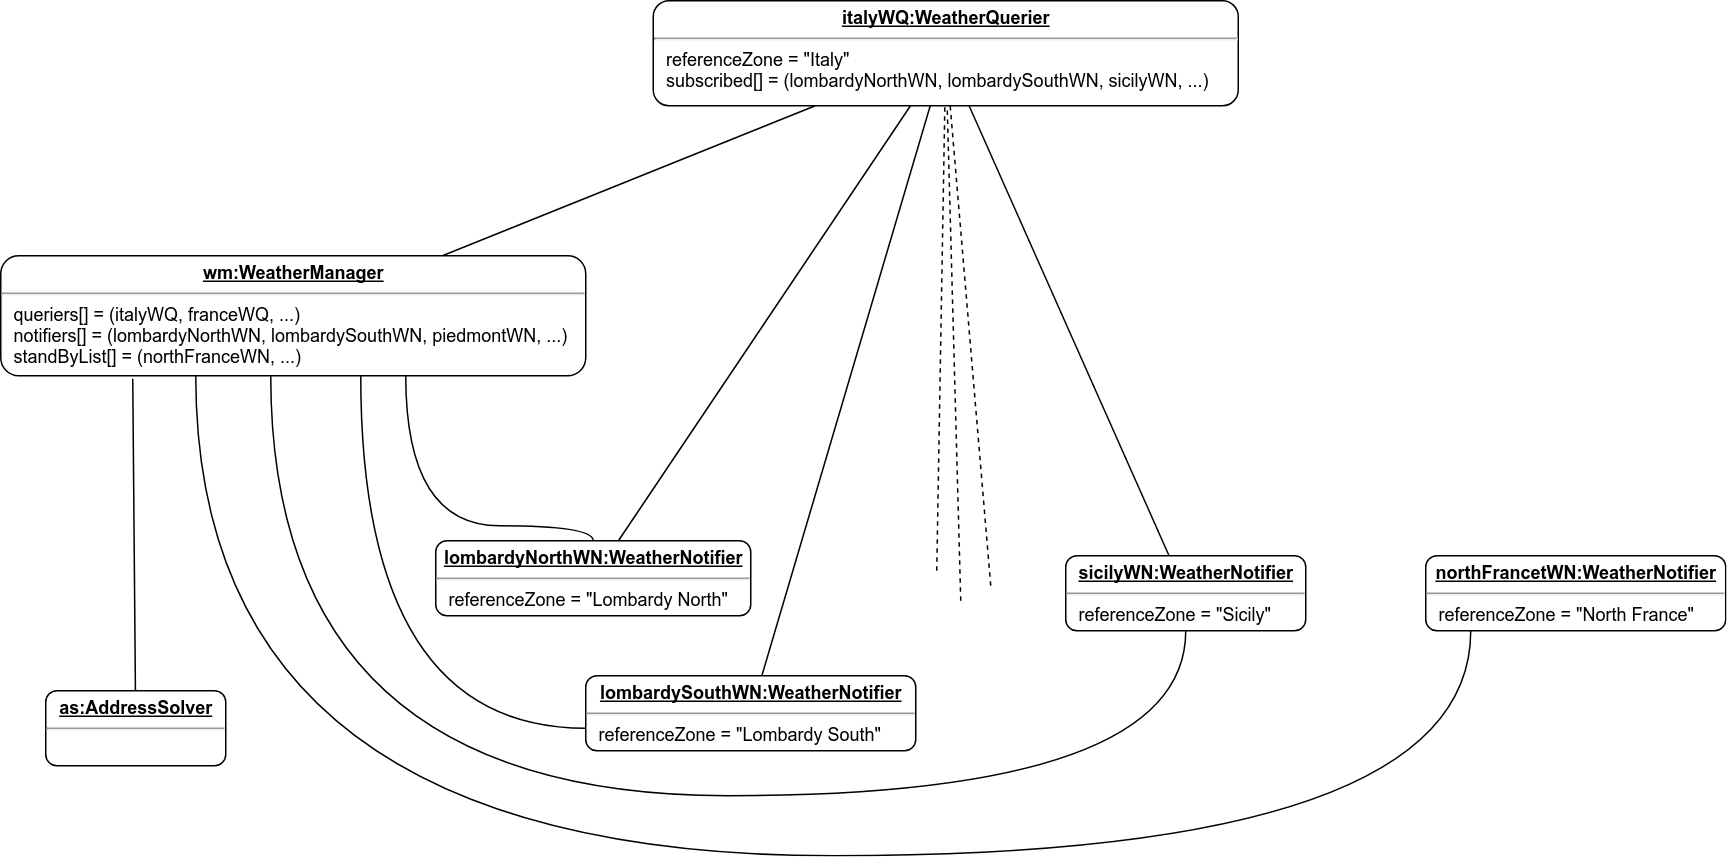
\includegraphics[width=0.9\paperwidth]{Images/OD_WeatherModule_After}}
			\caption{Object Diagram - Weather Module After Balancing and Reconfiguration}
		\end{figure}
\subsection{Component interfaces}
	% TODO
	
\subsection{Selected architectural styles and patterns}
	% TODO
	
\subsection{Other design decisions}
	% TODO